% !TeX spellcheck = en_US
\chapter{Prehľad algoritmov}
Na hľadanie najkratších ciest v grafe poznáme mnoho algoritmov, ktoré rozdeľujeme do týchto troch \cite{mares07} skupín: 


\begin{itemize}
\item Point To Point Shortest Path(P2PSP) - hľadajú najkratšiu cestu medzi dvoma zadanými bodmi.
\item Single Source Shortest Path(SSSP) - pre daný vrchol {\sl v} hľadajú najkratšiu cestu do všetkých vrcholov grafu.
\item All Pairs Shortest Path (APSP)- skúmajú najkratšiu cestu medzi všetkými dvojicami vrcholov.
\end{itemize}

Tieto problémy sú na obecných grafoch NP-ťažké.
Napriek tomu na mriežkových grafoch (kde sú vzdialenosti medzi vrcholmi vždy kladné) existujú algoritmy v polynomiálnom čase.

V práci budeme ďalej zaoberať riešením prvého problému (Point to Point Shortest Path). 

V tejto kapitole popíšeme algoritmy, ktoré sú použiteľné na grafoch s nezápornými dĺžkami hrán. TODO?? prerob

TODO?? POTIAL VSETKO PREPISANE a myslim, ze clekom prijemne citatelne.


\section{Kritéria efektivity algoritmu}
Na porovnanie efektivity algoritmou slúži v teoretickej informatike odhad asymptotickej složitosti \cite{asymptotic65}.
Tento odhad je veľmi užitočný v teoretickej informatike a veľmi často algoritmus s lepšou zložitosťou je v praxi rýchlejší.
Nie je to ale pravidlom a teda potrebujeme zaviesť ďalšie kritériá, ktoré presnejšie popíšu a porovnajú správanie algoritmov praxi.
Kritéria, podľa ktorých budeme porovnávať efektivitu algoritmov sú teda nasledovné:
\begin{itemize}
	\item Asymptotická zložitosť.
	\item Počet navštívených vrcholov.
	\item Reálny čas behu algoritmu.
\end{itemize}



\section{Dijkstrov algoritmus}
Medzi základné algoritmy typu SSSP patrí Dijkstrov algoritmus \cite{dijkstra59} popísaný už v roku 1959. 
Miernu modifikáciu pôvodného algoritmu môžeme vidieť na (Algoritmus \ref{alg:dijkstra}).  ASK?? spravil som citacie spravne?
Patrí medzi relaxačné algoritmy~a zbehne korektne na grafoch
s nezápornými hranami.

Pri hľadaní cesty z vrcholu $s$ do vrcholu $t$ prechádzame postupne vrcholy s neklesajúcou vzdialenosťou od $s$, až dokým sa nedostaneme k cieľovému vrcholu $t$.


ASK?? rozlisujeme tri stavy vrcholov, co je halda blablabla mam popisat aj slovne???

\begin{algorithm}
\caption{Dijkstra: nájdi najkratšiu cestu medzi dvoma bodmi $s$ a $t$}
\label{alg:dijkstra}
\begin{algorithmic}[1] % number one = line numbering is on
\REQUIRE graf $G$
\ENSURE dĺžková funkcia $d$ obsahujúca najkratšie cesty  z vrcholu $s$ do vrcholov grafu


\STATE $ d(*) \leftarrow \infty $
\STATE $ stav(*) \leftarrow$ NENAVŠTÍVENÝ

\COMMENT {pridám počiatok}
\STATE $d(s) \leftarrow 0$
\STATE $stav(s) \leftarrow $ OTVORENÝ
\STATE Heap $H$
\STATE $Insert(H, s)$

\WHILE {$H$  not empty}
	
	\STATE // vyberiem v -- najbližší otvorený vrchol
	\STATE $v \leftarrow ExtractMin(H)$
	
	\WHILE {$stav(v) \neq $ OTVORENÝ}
		\STATE $v \leftarrow ExtractMin(H)$
	\ENDWHILE
	
	\STATE // zrelaxujeme vrchol $v$
	\FORALL {$e$, $e = (v, u)$}
		\IF {$d(u) > d(v) + l(v, u)$}
			\STATE $Insert(H, v)$
			\STATE $stav(u) \leftarrow$ OTVORENÝ
			\STATE $d(u) \leftarrow d(v) + l(v, u)$
			
		\ENDIF
	\ENDFOR
\ENDWHILE

\end{algorithmic}
\end{algorithm}

\begin{theorem}
V dijkstrovom algoritme uzatvárame každý dosiahnuteľný vrchol práve raz.
\end{theorem}


\subsection{Zložitosť}
Na každý vrchol zavoláme operáciu $Insert$ maximálne $deg(v)$-krát a~teda počet všetkých zavolaní tejto operácie bude rádovo $\BigO{\sum_{v}{deg(v)}} = \BigO{m}$.
Zo štruktúry môžme vybrať maximálne toľko prvkov, koľko sme tam vložili a~teda aj volania $ExtractMin$ trvajú $\BigO{m}$.

Algoritmus teda zbehne v čase $\BigO{m T_i + m T_e}$, kde $T_i$ odpovedá času na vloženie prvku a $T_d$ odpovedá času na vybranie najmenšieho prvku.

To znamená, že zložitosť algoritmu závisí od zložitosti operácií $Insert$ a $ExtractMin$. Na riedke grafy je obecne v praxi najvýhodnejšie použiť 
binárnu haldu, ktorej obe operácie trvajú $\BigO{\log{n} } $ a celkový čas je teda $\BigO{m\log{n}}$
Prehľad štruktúr aj so zložitosťami operácií $Insert$ a $ExtractMin$ sa nachádza napr. na \cite{mares07}.

\subsection{Halda na mriežkovom grafe}
Nakoľko mriežkový graf je veľmi špeciálny typ grafu,
vieme niektoré jeho vlastnosti využiť na~to, aby sme vytvorili štruktúru, ktorá zvládne obe operácie v~konštantnom čase. 


Na konštrukciu tejto štruktúry (viď \cite{gs97}) budeme potrebovať nasledujúcu vetu.

\begin{theorem}
Pokiaľ sme v Dijkstrovom algoritme uzavreli vrchol $u$ so vzdialenosťou $d(u)$ a~najkratšia hrana v~grafe má dĺžku $\epsilon$, tak môžme taktiež 
uzavrieť všetky vrcholy $v$ so~vzdialenosťami $d(v) \in (d, d + \epsilon)$.
\end{theorem}
\begin{proof}
Do haldy vieme pridávať len vrcholy so vzdialenosťami aspoň $d + \epsilon$ (kratšia hrana tam už nie je), 
ale~tie už cestu k~vrcholom so~vzdialenosťami
$d_v \in (d, d + \epsilon)$ skrátiť nemôžu.
\end{proof}


\begin{consequence}
Keď uzavrieme vrchol so vzdialenosťou $d_u$, môžme uzavrieť aj vrcholy vo vzdialenosťami menšími, ako $d_u + \epsilon$
pričom poradie je nezávislé od skutočnej vzdialenosti vrcholov.
\end{consequence}

\begin{example}
\label{ex:range}
Dĺžka $\epsilon$ najkratšej hrany v mriežkovom grafe je 1. Je to dĺžka akejkoľvek vodorovnej, alebo zvislej hrany.
Keď teda uzavrieme vrchol so vzdialenosťou $d(u)$, môžme uzavrieť aj vrcholy so vzdialenosťami menšími, ako je $d(u) + 1$ a to v ľubovoľnom poradí.
\end{example}

Tieto veci vieme výborne využiť pri konštrukcii štruktúry
zvanej {\sl priehradková halda}. Tá, využijúc vyššieuvedenú vetu, uzatvára a pridáva vrcholy bez porušenia akejkoľvek konzistencie behu algoritmu.

ASK?? mam to supnut to kapitoly o 'mojom' algoritme?
Totizto o priehradkovej strukture sa da docitat vsade, neni
to moj patent, ale na druhu stranu ja som tu strukturu implenmentoval konkretne ma moj mriezkovy graf...


\subsection{Popis haldy}
Najprv popíšeme fungovanie haldy a graficky znázorníme jej 
operácie. Neskôr dokážeme, že keď túto haldu použijeme v Dijkstrovom algoritme, tak nám bude vraciať korektné výsledky.

Majme haldu s tromi priehradkami (nazvime ju $BucketHeap$), pričom rozsah jednej priehradky je ostro menší, ako 1.
Prvá priehradka uchováva prvky s rozsahom vzdialeností $ [b, b+1) $, druhá $ [b+1, b+2) $ a tretia $ [b+2, b+1+\sqrt{2}) $
pre danú bázu $ b $. Pre jednoduchšiu implementáciu $b \in \N$. Operácia $push((dist, data))$ vloží do haldy prvok so vzdialenosťou $dist$ 
s pomocnými dátami $data$. Operácia $pop()$ vracia ľubovoľný element z prvej priehradky. 
Pre jednoduchšiu implementáciu budeme mať na začiatku smerník na prvý prvok prvej priehradky a po vyhodení najmenšieho prvku tento smernik jednoducho inkrementujeme, kým to bude možné. Keď už v prvej priehradke nezostane žiaden prvok a zavoláme operáciu $pop()$, vykoná sa nasledujúca vec: druhú priehradku presunieme na miesto prvej, tretiu na miesto druhej a prvú dáme namiesto tretej.

Ilustrujme si to na obrázkových príkladoch. Príklad troj--priehradkovej haldy vidíme na obrázku \ref{fig:priehradky}.
ASK?? troj--priehradkovej? 
Halda uchováva premennú $ baza $, ktorá definuje bázu od ktorej sa rozsahy priehradok odvíjajú. Okrem
nej, uchováva tri smerníky na tri po sebe idúce priehradky priehradky a smerník na vrchol haldy, zvaný $ top $.



\begin{figure}[h]
\centering
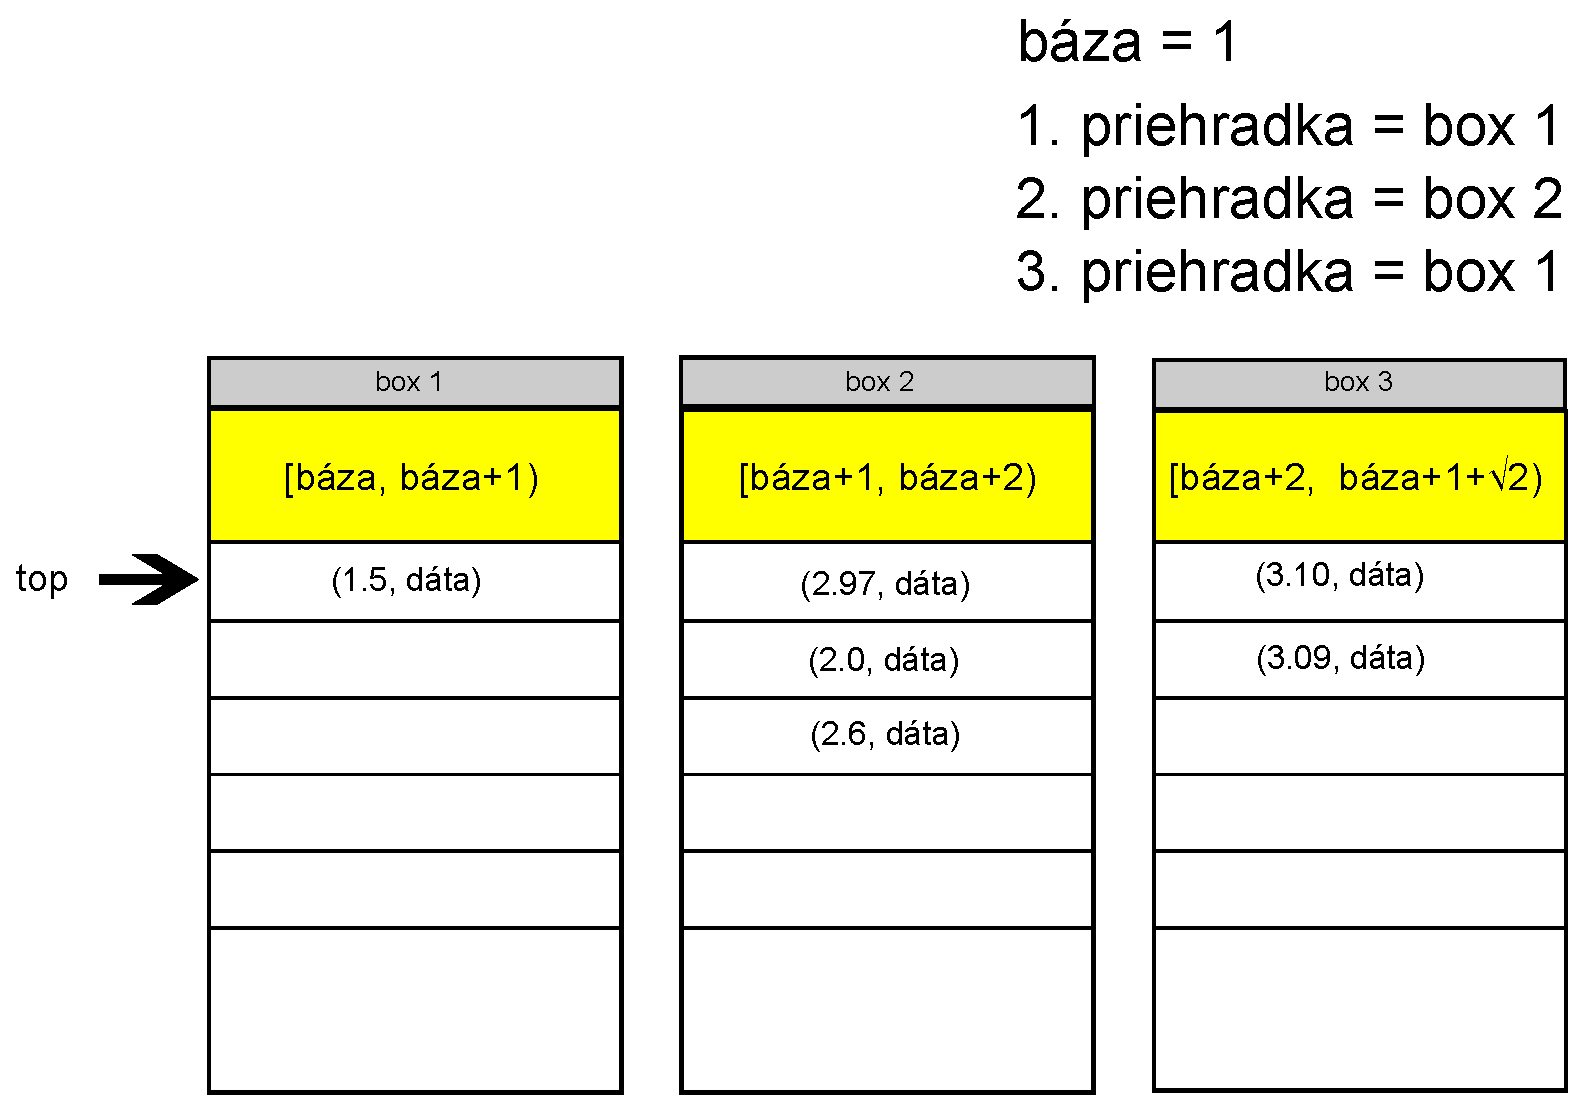
\includegraphics[width=\textwidth]{./img/priehradky_naplnene_default.eps}
\caption{Priehradky}
\label{fig:priehradky}
\end{figure}

Pridanie dvoch prvkov je znázornené na obrázku \ref{fig:priehradky_i}. Priehradka, do ktorej má byť prvok s danou vzdialenosťou vložený sa vypočíta podľa vzorca: $ \lfloor vzdialenostPrvku - baza +1 \rfloor $.


\begin{figure}[h]
\centering
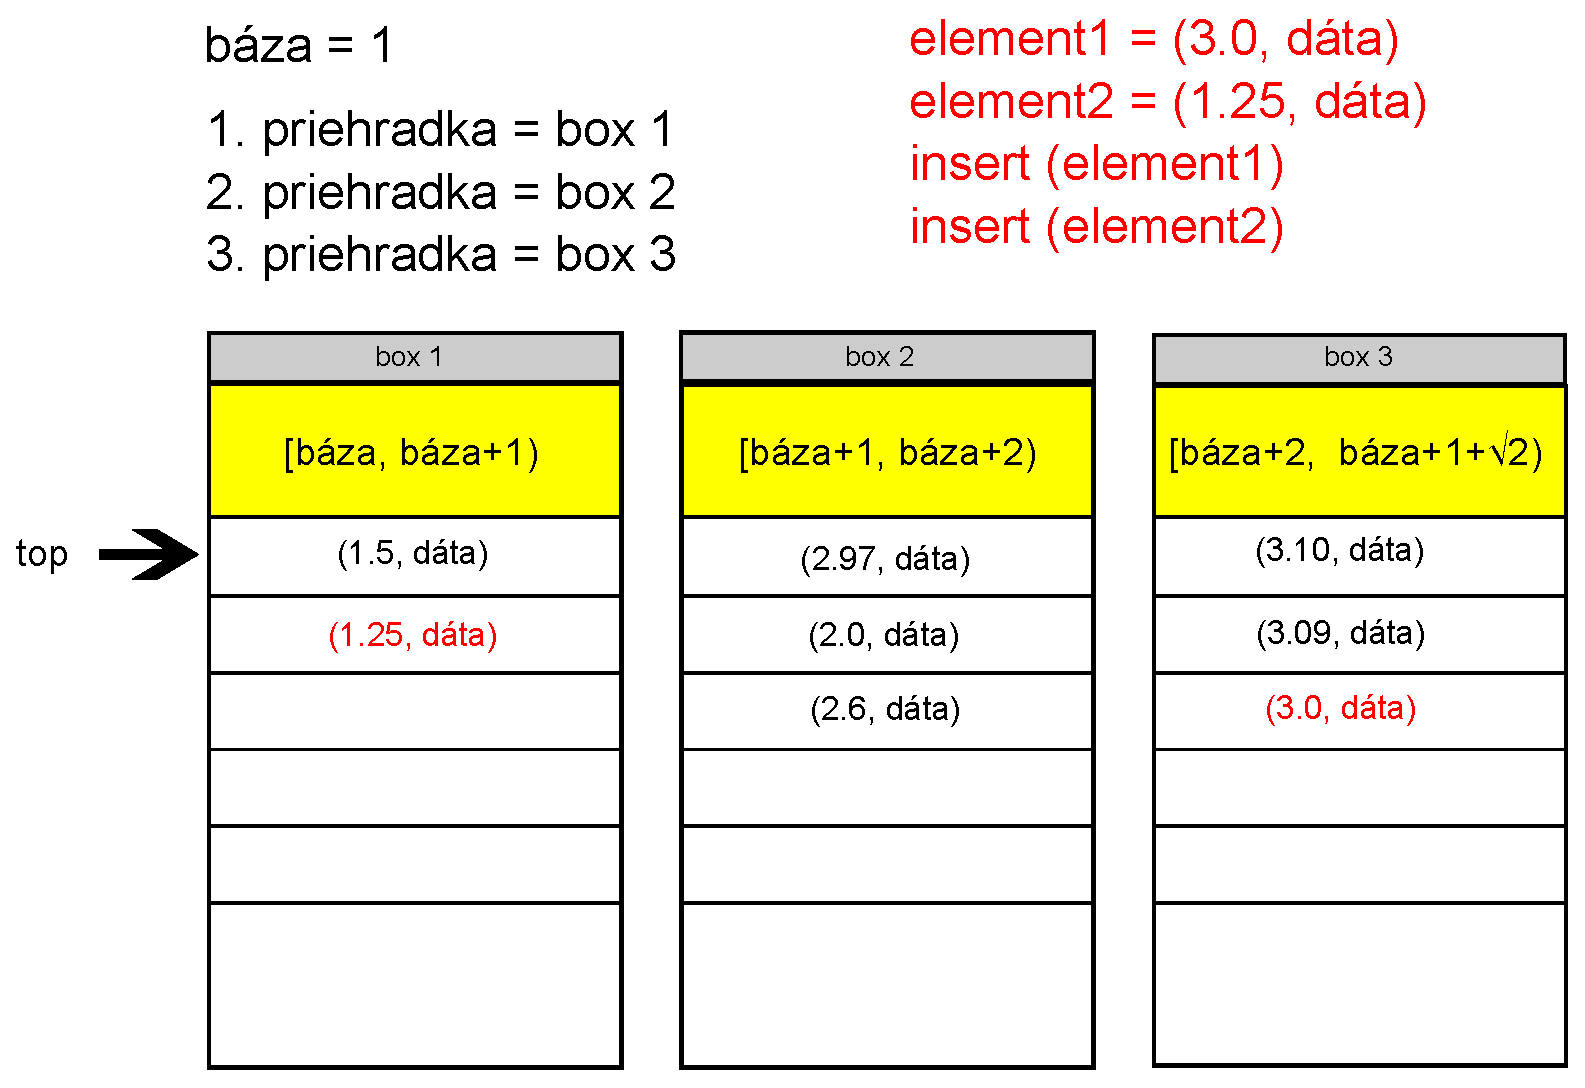
\includegraphics[width=\textwidth]{./img/priehradky_naplnene_default_i.eps}
\caption{Insert}
\label{fig:priehradky_i}
\end{figure}


Zmazanie prvku vidíme na obrázku \ref{fig:priehradky_i_d1}.
Celé zmazanie spočíva v inkrementácii ukazovateľa na vrch priehradky.

\begin{figure}[h]
\centering
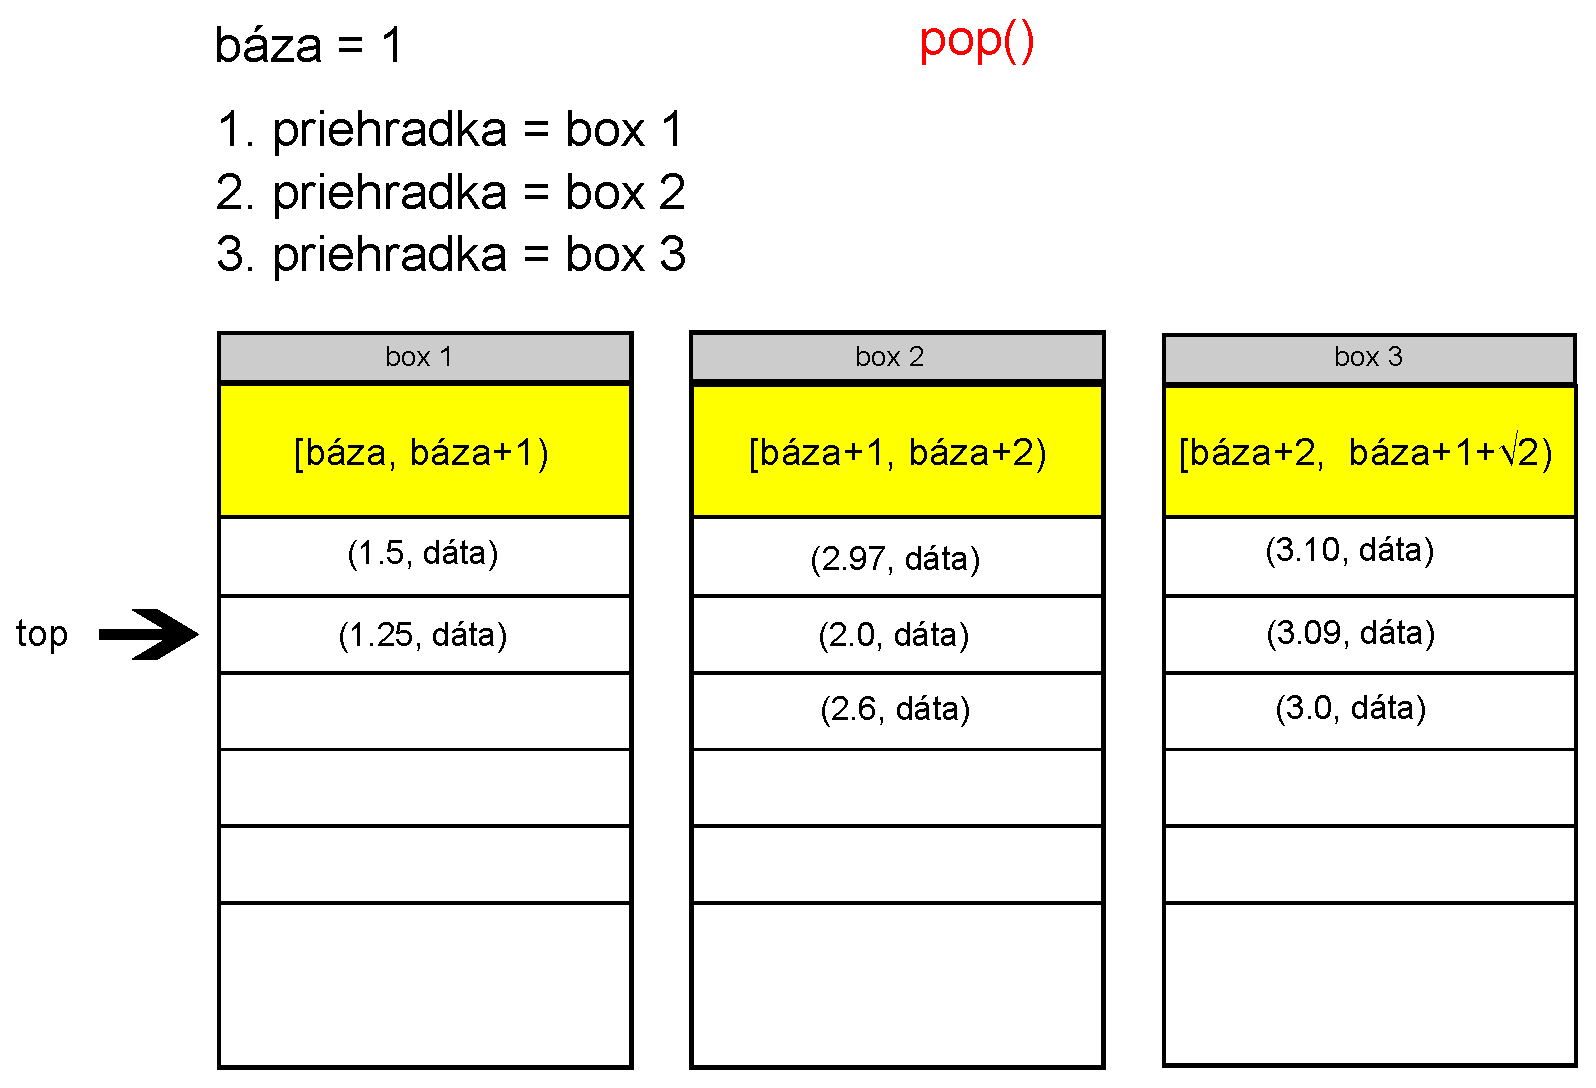
\includegraphics[width=\textwidth]{./img/priehradky_naplnene_default_i_d1.eps}
\caption{Pop (1)}
\label{fig:priehradky_i_d1}
\end{figure}


Pokiaľ sa v priehradke nachádza jediný prvok a ten chceme vybrať, tak nám inkrementácia premennej $ top $ v priehradke 
nepostačí. Musíme prehodiť priehradky. Druhú priehradku presunúť
na miesto prvej, tretiu na miesto druhej a prvú umiestniť nakoniec. Viď obrázok \ref{fig:priehradky_i_d2}. Nakoniec musíme zvýšit bázickú vzdialenosť. Zmena poradia týchto priehradok sa samozrejme uskutočňuje cez prehodenie smerníkov.
Keďže máme konštatný počet priehradok, tak aj táto operácia
trvá konštantný čas.

\begin{figure}[h]
\centering
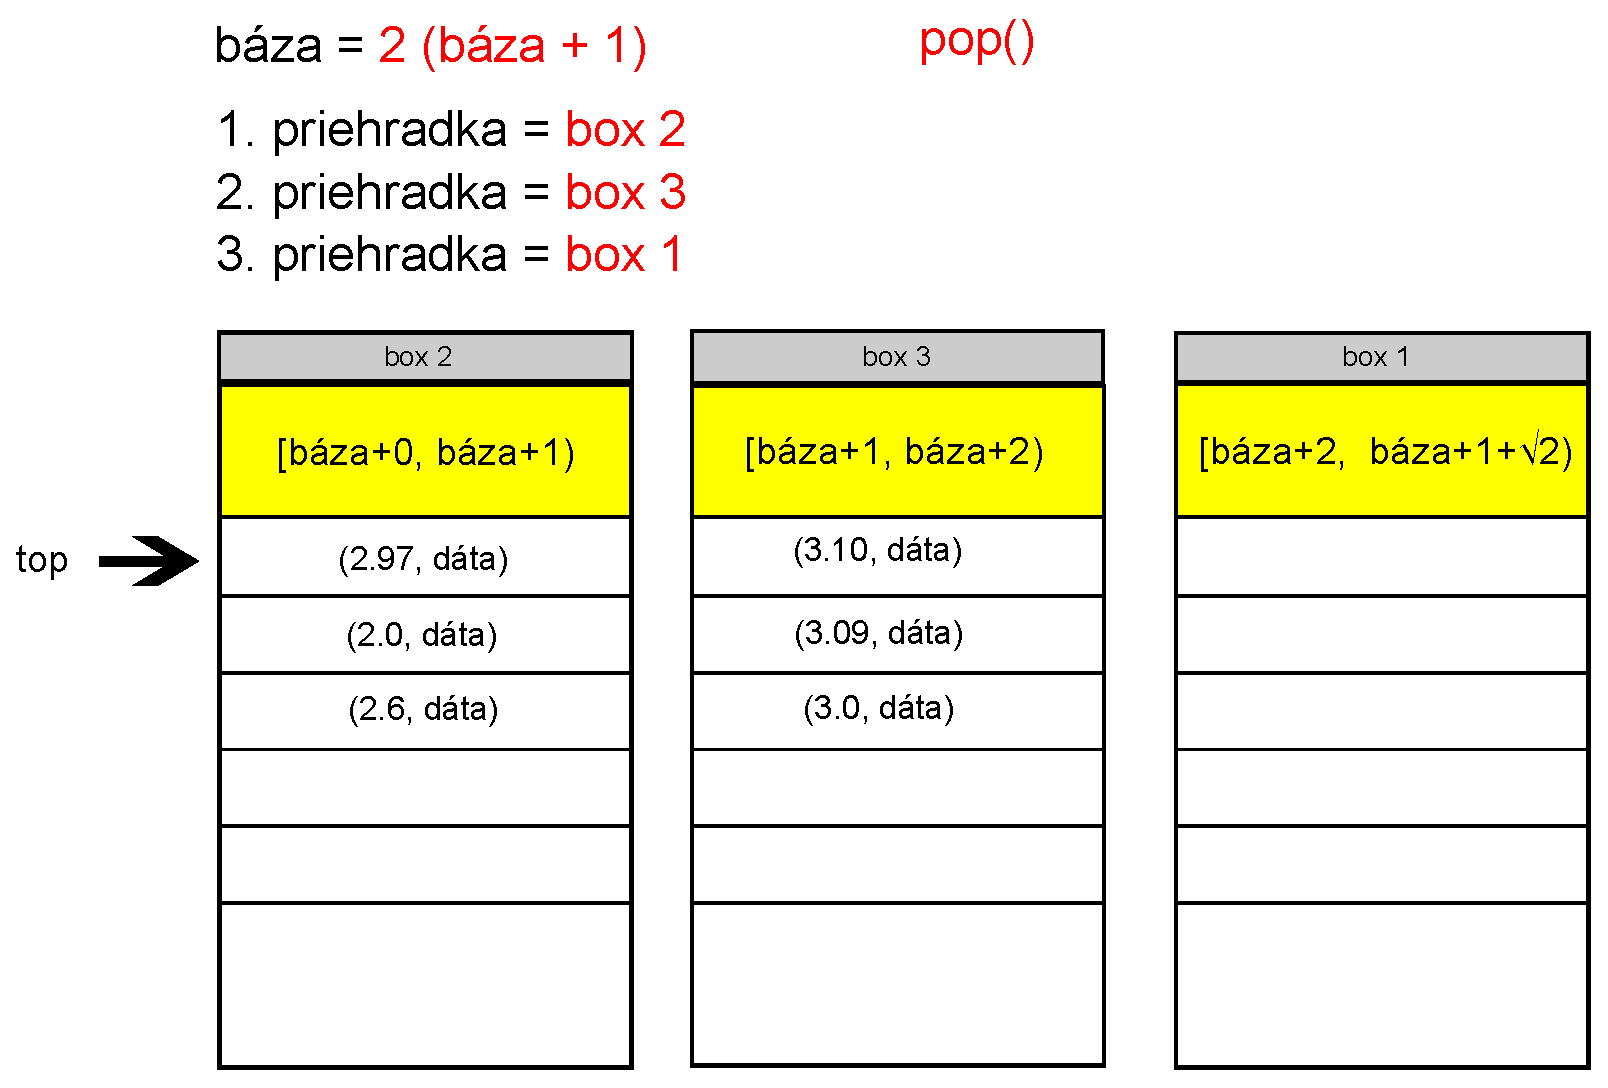
\includegraphics[width=\textwidth]{./img/priehradky_naplnene_default_i_d2.eps}
\caption{Pop (2)}
\label{fig:priehradky_i_d2}
\end{figure}


\begin{theorem}[korektnosť priehradkovej štruktúry]
Dijkstrov algoritmu používajúci haldu $BucketHeap$ vráti korektné najkratšie vzdialenosti do vrcholov grafu.
\end{theorem}
\begin{proof}
Rozsah každej priehradky je ostro menší, ako 1. To znamená, že podľa príkladu \ref{ex:range} operácia $pop()$ vracia prvky v poradí, ktoré
nepokazí chod algoritmu. 

Treba ešte dokázať, že tri priehradky postačujú. To je zrejmé,
pretože keď vyberieme vrchol z prvej priehradky, tak jeho vzdialenosť je v rozsahu $[b, b+1)$. Keď prechádzame jeho susedné vrcholy, tak najdlhšia hrana je $ \sqrt{2} $ a teda vzdialenosť k najvzdialenejšiemu susednému vrcholu je ostro menšia, ako $b+1+\sqrt{2}$.
\end{proof}


\section{A*}
Ďalší algoritmus, ktorým sa budeme zaoberať je algoritmus
A* \cite{astar72} prvykrát popísaný v roku 1968.

Tento algoritmus vychádza z Dijkstrovho algoritmu a je mu veľmi podobný. Hlavný rozdiel medzi týmito algoritmami je, že
kým Dijkstrov algoritmus vyberá z haldy vrcholy s neklesajúcou vzdialenosťou $ d(v) $ od počiatku, tak algoritmus A* vyberá prvky s neklesajúcou vzdialenosťou $ f(v) := d(s,v) + h(v,t) $, kde $ h(v, t) $ značí heuristickú funkciu, ktorá je dolným odhadom vzdialenosti od vrcholu $ v $ do cieľa $ t $. Obrátene, Dikstrov algoritmus si vieme predstaviť ako algoritmus A*, kde $ \forall v \in G: h(v, t) = 0 $.

Použitá heuristická funkcia má dopad na počet prehľadaných vrcholov a teda do zásadnej miery ovplyvňuje výkon algoritmu.

\subsection{Heuristická funkcia}
 Heuristická funkcia nemôže byť ľubovoľná. Funkcia musí predstavovať tzv. {\sl prípustný potenciál}. Podrobnejší popis sa nachádza napr. na \cite{mares07} \cite{golberg01} \cite{goldbergharrelson05}. Ďalej sa budeme venovať len funkciám, ktoré túto podmienku splňujú.


Najčastejšie heuristické funkcie sú tieto:

\begin{itemize}
\item Euklidovská vzdialenosť.
\item Trojuholníková nerovnosť, tzv. $ landmarks $.
\end{itemize}


\paragraph{Euklidovská vzdialenosť}

Euklidovská vzdialenosť je najjednoduchšie implementovateľná heuristická funkcia. Na väčšine jednoduchých grafov s malým počtom prekážok vracia dobré výsledky. Problém nastáva na grafoch, kde začiatok a koniec cesty sú geometricky blízko seba, hoci ich skutočná vzdialenosť je veľká.
Príklad vidíme na obrázku \ref{fig:antieuclid}.


\begin{figure}[h]
\centering
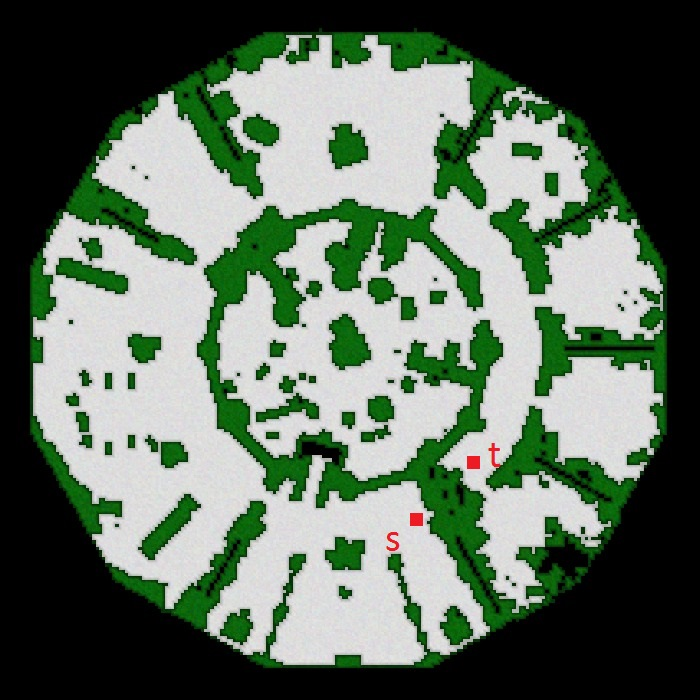
\includegraphics[width=0.5\textwidth]{./img/antieuclid505d.jpg}
\caption{Mapa, na ktorej euklidovská heuristika zlyhá.}
\label{fig:antieuclid}
\end{figure}


\paragraph{Landmarks a trojuholníková nerovnosť}
Nevýhoda použitia euklidovskej heuristickej funkcie je na obecných mapách zjavná. To motivovalo vymyslieť heuristiku, ktorá lepšie odráža vzdialenosti v grafe.

Jednou z týchto heuristík je počítanie dolného odhadu pomocou tzv. {\sl landmarks}. 

Landmarks sú vybrané vrcholy v grafe, z ktorých je následne prepočítaná najkratšia vzdialenosť do všetkych ostatných
vrcholov grafu. 



Kedže jeden prechod grafu vieme Dijkstrovým algoritmom s priehradkami vykonať za lineárny čas, predpočítanie $ k $ landmarkov trvá $ \BigO{kn} $, kde $n$ značí počet vrcholov grafu.


TODO?? ako to funguje...

\subparagraph{Možnosti voľby landmarkov}

Pri voľbe landmarkov sú dva faktory: počet a rozmiestnenie.

\begin{example}[na počte záleží]
Pokiaľ zvolíme málo landmarkov, tak dolný odhad nebude presný.
Pokiaľ ich zvolíme priveľa, tak prepočet vzdialenosti cez každý landmark pre každý vrchol zaberie veľa času.
\end{example}

\begin{example}[na rozmiestnení záleží]
Pokiaľ zvolíme všetky landmarky hneď pri sebe, tak heuristika
nám nebude vraciať dostatočne presné dolné odhady na vzdialenosť vrcholov, ktoré sú ďaleko od landmarkov.
\end{example}


ASK?? jak spravi dalsie hlbsie cislovanie odstavcov???







TODO??potencialy euklid landmarks landmark selection priblem s priehradkami